\chapter{Revisão de Literatura}
Esta seção apresentará os principais conceitos envolvidos na realização do trabalho como Cultivo em Ambiente Protegido, IoT, RSSF e também as tecnologias empregadas no desenvolvimento do trabalho, como sensores e atuadores.

\section{Cultivo em Ambiente Protegido}
Os fatores climáticos são uma das maiores preocupações do produtor, intempéries climáticas como geadas, excesso de chuvas, etc, prejudicam tanto a qualidade quanto o rendimento da produção. Para se contornar esses fatores uma alternativa a se considerar é o cultivo em ambientes protegidos, esta técnica possibilita um certo controle sobre as condições climáticas como temperatura, umidade do ar, etc \cite{silva2014cultivoprotegido}.

A forma de cultivo protegido mais conhecida é aquela realizado nas estufas, mas também pode ser efetuado por meio de túneis, ripados, etc.

\subsection{Nebulizador}

A nebulização, que é uma técnica que consiste na emissão de uma névoa de micro gotas de água, é indicado para climatização de ambientes onde se necessite o aumento da umidade relativa do ar e/ou abaixamento da temperatura em áreas de cultivo sob ambiente protegido, tais como viveiros e estufas. 

\begin{figure}[H]
\centering
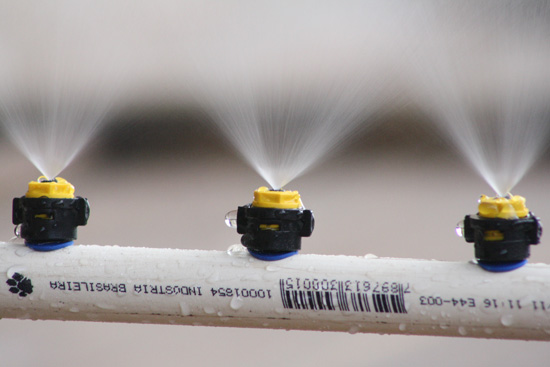
\includegraphics[scale=0.5]{04-figuras/nebulizador.jpg}
\begingroup
\caption{Sistema nebulizador}
\vspace{-\baselineskip}
\fonte{\url{https://www.growshop.com.br/media/wysiwyg/Close_Jato_NA-1_1.jpg}}
\label{fig:nebulizador}
\endgroup
\end{figure}

A nebulização também é utilizada na conservação de flores, estábulos, granjas, balcões de verduras em supermercados, entre outros. O controle do clima ou microclima nas estufas é baseado no princípio da troca de energia entre o ar e a água nebulizada, onde uma caloria representa a quantidade de calor necessária para aumentar em 1 °C a temperatura de 1 cm³ de água.

Em um sistema de nebulização eficiente pode se reduzir de 4 ºC a 6 ºC a temperatura na estufa, em relação às condições externas, ou seja, temperatura e umidade externa. A figura \ref{fig:nebulizador} mostra um sistema nebulizador.

\subsection{Setor de Fruticultura do campus Muzambinho}

No setor de fruticultura do IFSULDEMINAS campus Muzambinho é realizado o cultivo de mudas por estaquia. Esse cultivo é realizado em ambiente de cultivo protegido, como mostra a figura \ref{fig:fruticultura}. Este ambiente conta com um sistema de nebulizador responsável por controlar a temperatura e umidade do ar dentro do ambiente protegido.

O sistema nebulizador existente no setor é controlado por meio de um Arduino que efetua o acionamento de forma programada a cada 10 minutos.

\begin{figure}[H]
    \centering
    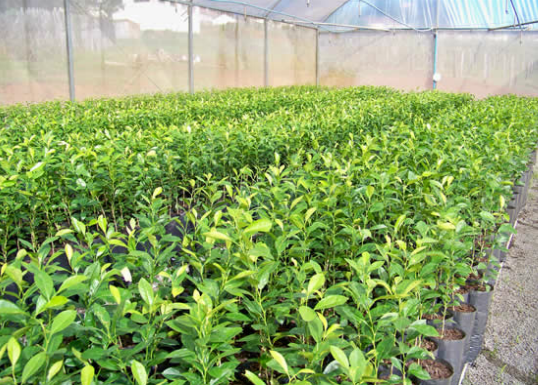
\includegraphics[scale=1]{04-figuras/fruticultura.png}
    \caption{Setor de fruticultura campus Muzambinho}
    \vspace{-\baselineskip}
    \fonte{Setor de Fruticultura do campus Muzambinho}
    \label{fig:fruticultura}
\end{figure}

\section{Internet das Coisas}

A Internet das Coisas (IoT, do inglês Internet of Things) vem se tornando algo comum em sociedade e visa conectar a vida cotidiana a objetos que possuem a internet como meio de comunicação. Essa interconexão de dispositivos na internet possibilita a comunicação dos mesmos com humanos ou até com outros dispositivos conectados \cite{leandro2017}.

\subsection{Rede de Sensores sem Fio}

Nos últimos anos, devido ao avanço tecnológico na área de sensores e comunicação sem fio, houve a criação das Redes de Sensores sem Fio (RSSF). Este tipo de rede pode atuar em diferentes atividades, como monitoramento, rastreamento, entre outras.

As redes de sensores sem fio se diferem das redes convencionais por serem compostas por diversos nos distribuídos além de possuir limitação quanto ao alcance e energia. Cada nó da rede é composto por diversos sensores tais como temperatura, infravermelho, pressão, etc, e esses nós podem ser organizados como \textit{clusters} onde pelo menos um nós seja capaz de detectar algum evento na região e comunicar este evento aos demais nós conectados na rede \cite{loureiro2003redes}.

\citeonline{rocha2007rede}, afirma que essas são algumas características que podem influenciar no projeto de uma rede de sensores sem fio:

\begin{itemize}[itemsep=0em]
    \item Tolerância a falhas: os sensores que compõem os nós são muito pequenos, o que contribui ao fato de eles serem pouco confiáveis, fazendo com que a rede tenha que ser tolerante a falhas. O nível de tolerância de falhas vai depender de cada aplicação. 
    \item Escalabilidade: o fato de os nós serem compostos por equipamentos de baixo custo e tamanho pequeno contribui para a criação de redes de alta escala, necessitando de poucos cuidados e baixo custo de instalação.
    \item Consumo de energia: a energia é um fator crucial em uma rede de sensores sem fio pois as fontes de energia são escassas. Dessa forma os nós devem usar a energia de forma eficiente, ficando "adormecidos" durante os períodos em que não forem necessários.
\end{itemize}

\section{Protocolo MQTT}

\textit{Message Queue Telemetry Transport} (MQTT), este protocolo foi desenvolvido pela IBM no final dos anos 90. 


\section{Microcontrolador}

Microcontroladores são dispositivos eletrônicos que possuem basicamente um microprocessador, memória e interfaces de entrada e saída. Estes dispositivos podem ser programados utilizando alguma linguagem de programação compatível, além de também poder trabalhar com diversos periféricos. Dito de outra forma

\begin{citacao}
	Microcontroladores são computadores de propósito específico. Eles possuem 
tamanho reduzido, baixo custo e baixo consumo de energia. Devido a esses fatores há diversos segmentos, que os utilizam, tais como a indústria automobilística, de telecomunicações, de brinquedos, de eletrodomésticos, de eletroeletrônicos, bélica [\ldots]. \cite{silva2009}  
\end{citacao}

De acordo com \citeonline[p.~15]{martins2005microcontroladores}, exitem diversos tipos de microcontroladores, sendo diferenciados por características como: a velocidade de processamento, a quantidade de memória disponível para armazenar dados e instruções, a quantidade de pinos de entrada e saída, entre outras.

\subsection{ESP8266} 

O modulo ESP8266 é um microcontrolador desenvolvido pela companhia Chinesa Espressif Systems.
O grande diferencial desse microcontrolador é possuir seu próprio sistema de comunicação WIFI, o que o faz ser grandemente utilizado como modulo WIFI por outros microcontroladores, como o Arduino por exemplo, apesar de possuir seu próprio processador, o que torna possível a criação de sistemas embarcados utilizando apenas o ESP8266 \cite[p.~26-27]{kolban2015espbook}.

A tabela \ref{tab:esp8266} mostra as especificações técnicas do ESP8266:

\begin{table}[H]
\centering
\caption{Especificações técnicas do ESP8266}
\begin{tabular}{c|c}
\hline
Voltagem 						& 3.3V 					\\\hline
Consumo de corrente 			& 10uA 					\\\hline
Memória Flash 					& 16MB max				\\\hline
Processador 					& Tensilica L106 32bit	\\\hline
Velocidade do Processador 		& 80-160MHz				\\\hline
RAM 							& 32K + 80K 			\\\hline
GPIOs 							& 17		 			\\\hline
Analógico para digital 			& 1 (1024 de resolução)	\\\hline
Suporte 802.11 					& b/g/n/d/e/i/k/r		\\\hline
Máxima corrente de conexão TCP	& 5						\\\hline
\end{tabular}
\label{tab:esp8266}
\fonte{\cite[p.27]{kolban2015espbook}}
\end{table}


\subsection{ESP-12}

Este módulo possui mais entradas e saídas, o que possibilita a leitura de vários sensores, sendo o ideal para compor um nó da rede de sensores.

\begin{figure}[H]
\centering
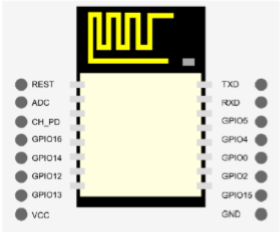
\includegraphics[scale=1]{./04-figuras/esp-12.png}
\begingroup
\caption{GPIOs do ESP-12}
\vspace{-\baselineskip}
\label{fig:esp12-gpios}
\fonte{\cite[p.29]{kolban2015espbook}}
\endgroup
\end{figure}

A figura \ref{fig:esp12-gpios} mostra o posicionamento de cada um dos pinos no ESP-12, as especificações e particularidades de cada um deles é apresentado na tabela \ref{tab:esp12-especificacoes}.

\begin{table}[H]
\centering
\caption{Especificações dos GPIOs}
\label{tab:esp12-especificacoes}
\begin{tabular}{l|l}
\hline
\multicolumn{1}{c|}{\textbf{Nome}} & \multicolumn{1}{c}{\textbf{Descrição}}                                                                                                                     \\ \hline
VCC                                 & 3.3V                                                                                                                                                        \\ \hline
GPIO 13                             & Pode ser usado como SPI MOSI                                                                                                                                \\ \hline
GPIO 12                             & Pode ser usado como SPI MOSI                                                                                                                                \\ \hline
GPIO 14                             & Pode ser usado como SPI MOSI                                                                                                                                \\ \hline
GPIO 16                             &                                                                                                                                                             \\ \hline
CH\_PD                              & \begin{tabular}[c]{@{}l@{}}Enable do ESP8266\\ Nível lógico 1 - Ativado\\ Nível lógico 0 - Desativado\end{tabular}                                          \\ \hline
ADC                                 & Entrada analógico para digital                                                                                                                              \\ \hline
Reset                               & \begin{tabular}[c]{@{}l@{}}1 - Normal\\ 0 - Reset\end{tabular}                                                                                              \\ \hline
TXD                                 & Transmissão serial                                                                                                                                          \\ \hline
RXD                                 & Recepção serial                                                                                                                                             \\ \hline
GPIO 4                              & GPIO normal                                                                                                                                                 \\ \hline
GPIO 5                              & GPIO normal                                                                                                                                                 \\ \hline
GPIO 0                              & \begin{tabular}[c]{@{}l@{}}Deve estar em nível lógico 1 para inicialização do programa (boot mode)\\ e 0 para carregar o programa (flash mode)\end{tabular} \\ \hline
GPIO 2                              & Deve estar em nível lógico 1 para inicialização do programa (boot mode)                                                                                     \\ \hline
GPIO 15                             & \begin{tabular}[c]{@{}l@{}}Deve estar em nível lógico 0 para carregar o programa (flash mode)\\ e para inicialização do programa (boot mode)\end{tabular}   \\ \hline
GND                                 & Terra                                                                                                                                                       \\ \hline
\end{tabular}
\fonte{\cite[p.29]{kolban2015espbook}}
\end{table}

\subsection{Plataforma NodeMCU}

NodeMCU é uma plataforma \textit{Open Source} baseado no microcontrolador ESP8266. Basicamente essa plataforma é composta por um microcontrolador (ESP8266, ESP-12) e uma porta micro USB utilizada para alimentação e programação da placa. Principais características do NodeMCU:
\begin{itemize}[itemsep=0em]
\item Processador ESP8266-12E
\item Arquitetura RISC de 32 bits
\item Processador pode operar em 80MHz ou 160MHz
\item 4Mb de memória flash
\item 64Kb para instruções
\item 96Kb para dados
\item WiFi nativo padrão 802.11b/g/n
\item Opera em modo AP, \textit{Station} ou AP + \textit{Station}
\item Pode ser alimentada com 5VDC através do conector micro USB
\item Possui 11 pinos digitais
\item Possui 1 pino analógico com resolução de 10 bits
\item Pinos digitais, exceto o D0 possuem interrupção, PWM, I2C e one wire
\item Pinos operam em nível lógico de 3.3V
\item Pinos não tolerantes a 5V
\item Possui conversor USB Serial integrado
\item Programável via USB ou WiFi (OTA)
\item Compatível com a IDE do Arduino
\item Compatível com módulos e sensores utilizados no Arduino
\end{itemize}

A figura \ref{fig:nodemcu} apresenta uma breve descrição da composição da placa:

\begin{figure}[H]
\centering
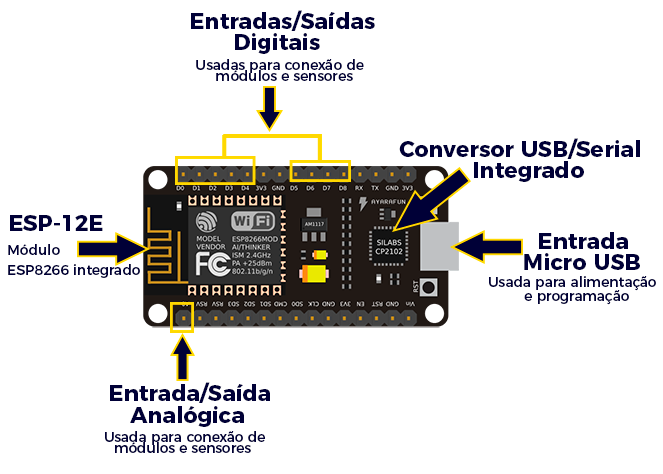
\includegraphics[scale=0.5]{./04-figuras/nodemcu.png}
\caption{Composição do NodeMCU}
\vspace{-\baselineskip}
\fonte{https://goo.gl/VAK2kx}
\label{fig:nodemcu}
\end{figure}

% Falar sobre o Gpio e a programação do nodeMCU

\section{Sensores}

Os sensores são dispositivos que respondem a interações com o ambiente. "Estes dispositivos podem interagir com diversos tipos de grandezas físicas, tais como temperatura, movimento, pressão, entre outras, convertendo essas grandezas em sinais elétricos analógicos ou digitais". \cite{marchesan2012sensores}.

\subsection{Sensor de Temperatura e Umidade do Ar}

O sensor de umidade do ar e temperatura escolhido pra utilização no desenvolvimento do trabalho foi o DHT11, representado na figura \ref{fig:dht11}, que é um sensor comercial de baixo custo. Este sensor utiliza um termistor para medição da temperatura e um sensor capacitivo para medir a umidade do ar \cite{gay2014dht11}.

Características do DHT11:
\begin{itemize}[itemsep=0em]
\item Tensão de alimentação de 3V a 5V
\item Tensão de alimentação máxima 5,5V
\item Corrente de operação 200uA a 500mA
\item Corrente de Stand-By 100uA a 150uA
\item Faixa de medição de umidade 0\% a 90\% com precisão de 5\%
 pra mais ou pra menos
\item Faixa de medição de temperatura 0ºC a 50ºC com precisão de 2\% pra mais ou para menos
\item Tempo de resposta <5s
\item Dimensões 23 x 12 x 5mm (incluindo os terminais)
\end{itemize}

\begin{figure}[H]
\centering
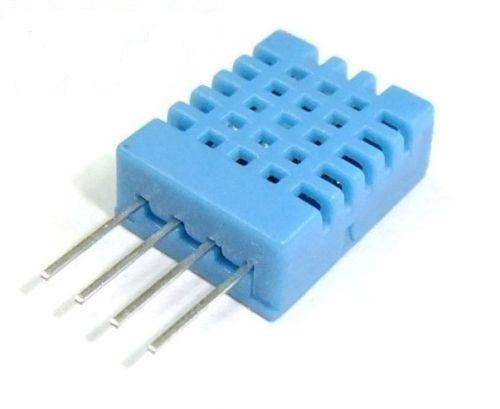
\includegraphics[scale=0.3]{./04-figuras/sensor_DHT11.jpg}
\caption{Sensor de umidade e temperatura}
\vspace{-\baselineskip}
\fonte{Do autor}
\label{fig:dht11}
\end{figure}


\subsection{Sensor de Molhamento Foliar}

Os sensores do tipo resistivo são comumente empregados para medição da duração do molhamento foliar, quando há água em sua superfície a resistência elétrica é reduzida devido a um curto-circuito proveniente da presença do líquido. Estes tipos de sensores são capazes apenas de detectar se há ou não água sobre a sua superfície, se precisarmos quantificar esse liquido será necessário a utilização de um sensor do tipo capacitivo.

Os sensores do tipo capacitivo trabalham da seguinte maneira:
\begin{itemize}[itemsep=0em]
\item quando não há a presença de nenhum liquido, o seu dielétrico é apenas o ar
\item conforme sua superfície entra em contato com algum líquido, parte do seu dielétrico se torna a água, que possui permissividade aproximadamente 80 vezes maior do que a do ar, provocando assim um aumento na capacitância. 
\end{itemize}
Dessa forma, ao medirmos a capacitância do sensor, poderemos estimar a quantidade de água que se encontra em sua superfície.
A figura \ref{fig:molhamento} mostra o sensor de molhamento foliar utilizado no trabalho.

\begin{figure}[H]
\centering
\setlength\lineskip{0pt}
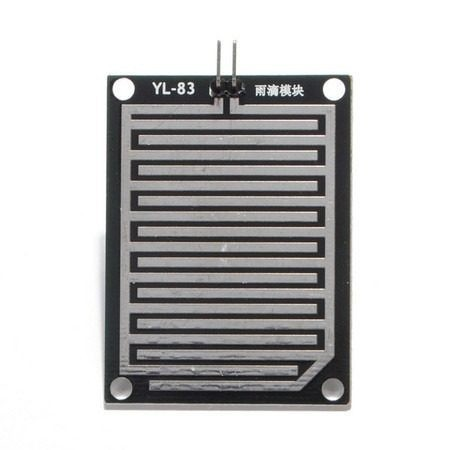
\includegraphics[scale=0.3]{./04-figuras/molhamento.jpg}
\caption{Sensor de Molhamento Foliar}
\vspace{-\baselineskip}
\fonte{Do autor}
\label{fig:molhamento}
\end{figure}

\begin{comment}
\subsection{Sensor de Luminosidade}

\textit{Light Dependant Resistor} (LDR) como mostra a figura \ref{fig:ldr} é um resistor cuja sua resistência varia de forma inversamente proporcional a incidência de luz, ou seja, quanto maior a iluminação menor será o valor da resistência \cite[p.114]{mcroberts2011arduinobasico}.

\begin{figure}[H]
\centering
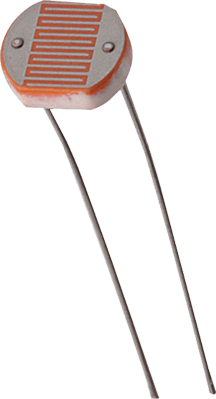
\includegraphics[scale=0.3]{./04-figuras/ldr.png}
\caption{Sensor de luminosidade (LDR)}
\vspace{-\baselineskip}
\fonte{Do autor}
\label{fig:ldr}
\end{figure}

Na tabela \ref{tab:vout-ldr} podemos constatar a variação dos valores de tensão de saída (Vout), indo de mais escuro para mais claro, para um LDR com tensão de entrada (Vin) de 5V e resistência de 10k$\Omega$ como divisor de tensão.

\begin{table}[H]
\centering
\caption{Valores de Vout (voltagem de saída) para um LDR com 5V como Vin (voltagem de entrada)}
\begin{tabular}{c|c|c|c}
\hline
\textbf{R1} & \textbf{R2 (LDR)} & \textbf{Vout} & \textbf{Claridade} 	\\\hline
10k$\Omega$ & 100k$\Omega$ 		& 4,54V 		& Mais escuro			\\\hline
10k$\Omega$ &  73k$\Omega$ 		& 4,39V 		& 25\%					\\\hline
10k$\Omega$ &  45k$\Omega$ 		& 4,09V 		& 50\%    				\\\hline
10k$\Omega$ &  28k$\Omega$ 		& 3,68V 		& 75\%    				\\\hline
10k$\Omega$ &  10k$\Omega$ 		& 2,50V 		& Mais claro    		\\\hline
\end{tabular}
\fonte{\citeonline[p.~119]{mcroberts2011arduinobasico}}
\label{tab:vout-ldr}
\end{table}
\end{comment}

\section{Atuadores}

Os atuadores são componentes que convertem energia, seja ela elétrica, hidráulica ou pneumática, em grandeza física, como movimento, calor, etc. Além disso os atuadores "atendem a comandos que podem ser manuais ou automáticos, ou seja, qualquer elemento que realize um comando recebido de outro dispositivo, com base em uma entrada ou critério a ser seguido". \cite{brugnari2010automaccao}

\subsection{Relé}

Relé é uma chave eletrônica que liga ou desliga quando recebe uma tensão em seus pinos de controle. Esta chave trabalha de forma diferente das convencionais pois não depende da intervenção humana para o seu acionamento \cite[p.28]{ribeiro1999automaccao}.

A figura \ref{fig:rele} representa a estrutura interna de um relé:

\begin{figure}[H]
\centering
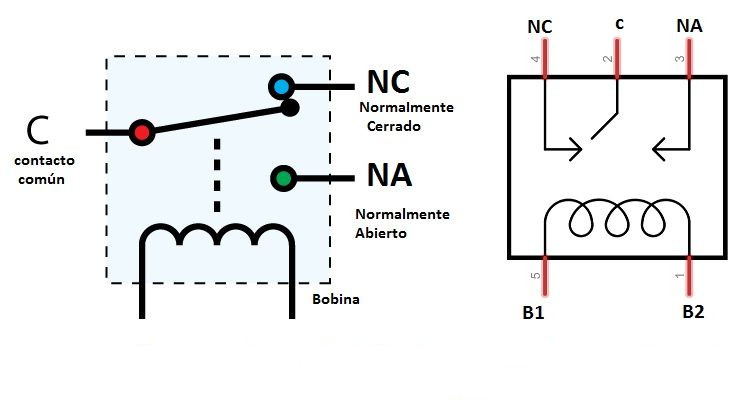
\includegraphics[scale=0.3]{./04-figuras/reles.jpg}
\caption{Estrutura interna do rele}
\vspace{-\baselineskip}
\fonte{http://www.areatecnologia.com/electricidadrele.html}
\label{fig:rele}
\end{figure}

\begin{itemize}[itemsep=0em]
\item B1 e B2 que são os terminais de controle, estes terminais são conectados à uma bobina que quando energizada fecha contato permitindo a passagem de corrente do pino C para o pino NO.
\item \textit{Normally Open} (NO) - normalmente aberto: quando o relé é acionado permite-se passagem de corrente do pino C para o NO.
\item \textit{Normally Close} (NC) - normalmente fechado: quando o relé é acionado passagem de corrente do pino C para o NC é interrompida.
\item \textit{Common Connection} (C) - conexão comum: terminal que é  conectado à fonte externa quando. Normalmente conectado ao pino NC, quando o rele é acionado a conexão é trocada para o pino NO.
\end{itemize}

\begin{figure}[H]
\centering
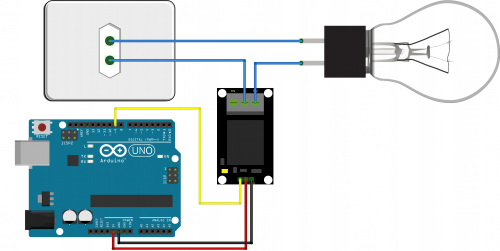
\includegraphics[scale=0.5]{./04-figuras/rele-exemplo.png}
\caption{Exemplo de ligação do rele com o Arduino}
\vspace{-\baselineskip}
\fonte{https://www.robocore.net/tutoriais/modulo-rele-arduino.html}
\label{fig:releligacao}
\end{figure}

A figura \ref{fig:releligacao} nos mostra um exemplo de ligação de um rele à plataforma Arduino, este rele está sendo utilizado para acionar uma lâmpada. Como podemos ver, esta lâmpada está conectada a uma fonte de energia externa, o papel do rele é trabalhar como uma chave que, ao receber uma tensão enviada pelo Arduino, permite a passagem da corrente, que vem da fonte externa, para a lâmpada.